\documentclass[journal,12pt,twocolumn]{IEEEtran}

\usepackage{setspace}
\usepackage{gensymb}
\singlespacing
\usepackage[cmex10]{amsmath}
\usepackage{float}
\usepackage{amsthm}
\usepackage{askmaps}
\usepackage{mathrsfs}
\usepackage{txfonts}
\usepackage{stfloats}
\usepackage{bm}
\usepackage{cite}
\usepackage{cases}
\usepackage{subfig}

\usepackage{longtable}
\usepackage{multirow}

\usepackage{enumitem}
\usepackage{mathtools}
\usepackage{steinmetz}
\usepackage{tikz}
\usepackage{circuitikz}
\usepackage{verbatim}
\usepackage{tfrupee}
\usepackage[breaklinks=true]{hyperref}
\usepackage{graphicx}
\usepackage{tkz-euclide}

\usetikzlibrary{calc,math}
\usepackage{listings}
    \usepackage{color}                                            %%
    \usepackage{array}                                            %%
    \usepackage{longtable}                                        %%
    \usepackage{calc}                                             %%
    \usepackage{multirow}                                         %%
    \usepackage{hhline}                                           %%
    \usepackage{ifthen}                                           %%
    \usepackage{lscape}     
\usepackage{multicol}
\usepackage{chngcntr}

\DeclareMathOperator*{\Res}{Res}

\renewcommand\thesection{\arabic{section}}
\renewcommand\thesubsection{\thesection.\arabic{subsection}}
\renewcommand\thesubsubsection{\thesubsection.\arabic{subsubsection}}

\renewcommand\thesectiondis{\arabic{section}}
\renewcommand\thesubsectiondis{\thesectiondis.\arabic{subsection}}
\renewcommand\thesubsubsectiondis{\thesubsectiondis.\arabic{subsubsection}}


\hyphenation{op-tical net-works semi-conduc-tor}
\def\inputGnumericTable{}                                 %%

\lstset{
%language=C,
frame=single, 
breaklines=true,
columns=fullflexible
}
\begin{document}


\newtheorem{theorem}{Theorem}[section]
\newtheorem{problem}{Problem}
\newtheorem{proposition}{Proposition}[section]
\newtheorem{lemma}{Lemma}[section]
\newtheorem{corollary}[theorem]{Corollary}
\newtheorem{example}{Example}[section]
\newtheorem{definition}[problem]{Definition}

\newcommand{\BEQA}{\begin{eqnarray}}
\newcommand{\EEQA}{\end{eqnarray}}
\newcommand{\define}{\stackrel{\triangle}{=}}
\bibliographystyle{IEEEtran}
\raggedbottom
\setlength{\parindent}{0pt}
\providecommand{\mbf}{\mathbf}
\providecommand{\pr}[1]{\ensuremath{\Pr\left(#1\right)}}
\providecommand{\qfunc}[1]{\ensuremath{Q\left(#1\right)}}
\providecommand{\sbrak}[1]{\ensuremath{{}\left[#1\right]}}
\providecommand{\lsbrak}[1]{\ensuremath{{}\left[#1\right.}}
\providecommand{\rsbrak}[1]{\ensuremath{{}\left.#1\right]}}
\providecommand{\brak}[1]{\ensuremath{\left(#1\right)}}
\providecommand{\lbrak}[1]{\ensuremath{\left(#1\right.}}
\providecommand{\rbrak}[1]{\ensuremath{\left.#1\right)}}
\providecommand{\cbrak}[1]{\ensuremath{\left\{#1\right\}}}
\providecommand{\lcbrak}[1]{\ensuremath{\left\{#1\right.}}
\providecommand{\rcbrak}[1]{\ensuremath{\left.#1\right\}}}
\theoremstyle{remark}
\newtheorem{rem}{Remark}
\newcommand{\sgn}{\mathop{\mathrm{sgn}}}
\providecommand{\abs}[1]{\left\vert#1\right\vert}
\providecommand{\res}[1]{\Res\displaylimits_{#1}} 
\providecommand{\norm}[1]{\left\lVert#1\right\rVert}
%\providecommand{\norm}[1]{\lVert#1\rVert}
\providecommand{\mtx}[1]{\mathbf{#1}}
\providecommand{\mean}[1]{E\left[ #1 \right]}
\providecommand{\fourier}{\overset{\mathcal{F}}{ \rightleftharpoons}}
%\providecommand{\hilbert}{\overset{\mathcal{H}}{ \rightleftharpoons}}
\providecommand{\system}{\overset{\mathcal{H}}{ \longleftrightarrow}}
	%\newcommand{\solution}[2]{\textbf{Solution:}{#1}}
\newcommand{\solution}{\noindent \textbf{Solution: }}
\newcommand{\cosec}{\,\text{cosec}\,}
\providecommand{\dec}[2]{\ensuremath{\overset{#1}{\underset{#2}{\gtrless}}}}
\newcommand{\myvec}[1]{\ensuremath{\begin{pmatrix}#1\end{pmatrix}}}
\newcommand{\mydet}[1]{\ensuremath{\begin{vmatrix}#1\end{vmatrix}}}
\numberwithin{equation}{subsection}
\makeatletter
\@addtoreset{figure}{problem}
\makeatother
\let\StandardTheFigure\thefigure
\let\vec\mathbf
\renewcommand{\thefigure}{\theproblem}
\def\putbox#1#2#3{\makebox[0in][l]{\makebox[#1][l]{}\raisebox{\baselineskip}[0in][0in]{\raisebox{#2}[0in][0in]{#3}}}}
     \def\rightbox#1{\makebox[0in][r]{#1}}
     \def\centbox#1{\makebox[0in]{#1}}
     \def\topbox#1{\raisebox{-\baselineskip}[0in][0in]{#1}}
     \def\midbox#1{\raisebox{-0.5\baselineskip}[0in][0in]{#1}}
\vspace{3cm}
\title{Design of FIR Low Pass Filter using Vaman }
\author{Priyanka - EE21MTECH12002}
\maketitle
\newpage
\bigskip
\renewcommand{\thefigure}{\theenumi}
\renewcommand{\thetable}{\theenumi}
Download all codes from 
\begin{lstlisting}
https://github.com/PeriPriyanka/FPGA_5811/Project/codes
\end{lstlisting}
\section{Design of fir filter using vaman}
FIR filter are Finite impulse response filters. The impulse response of the FIR is for finite duration of time.  The filter of infinite impulse response needs to truncate to finite impulse response. One of the methods for truncation is applying a window.  Windowing can be considered as a sort of amplitude envelope that gets multiplied with infinite impulse response to give finite impulse response. 
\begin{align}
h(n) = h_d(n) * w(n) 
\end{align}
Where, 
h(n) is finite impulse response,
$h_d(n)$ is infinite impulse response,
w(n) is window function.
\subsection{Steps to design a low pass filter}
\begin{enumerate}
\item Design an Infinite impulse response low pass filter.
\begin{align}
h_d (n) = \begin{cases} 
      \frac{\sin(w_c n)}{\pi n} & n = -\frac{(N-1)}{2} \text{ to } \frac{N-1}{2} \\ \\
      \frac{w_c}{\pi} & n=0 
   \end{cases} 
\end{align}
\begin{center}
or
\end{center}
\begin{align}
h_d (n) = \begin{cases} 
      \frac{\sin(w_c (n-\tau)}{\pi (n-\tau)} & n = 0 \text{ to } (N-1) \\ \\
      \frac{w_c}{\pi} & n=\tau 
   \end{cases} 
\end{align}
where center of symmetry, $\tau$ = (N-1)/2 and $w_c$ is digital cutoff frequency.
\item Design of a Hamming window
\begin{align}
w_h(n) = \begin{cases} 
     0.54 - 0.46 \cos(\frac{2\pi n}{N-1}) & n=0 \text{ to } N - 1 \\ \\
      0.54 + 0.46 \cos(\frac{2\pi n}{N-1}) & n = -\frac{(N-1)}{2} \text{ to } \frac{N-1}{2}
   \end{cases} 
\end{align}
\item Design a finite impulse response low pass filter
\begin{align}
h(n) = h_d(n) * w_h(n)
\end{align}
\end{enumerate}
\section{Design of filter in vaman}
An FIR Low pass filter designed by accessing the cutoff frequency from ESP32. ESP32 accesses the cutoff frequency from web server through WiFi module and passes the data to arm. Arm has been coded in a way to access the data from ESP32, produce the filter coefficients and returns the data to ESP32 via UART Serial communication. The ESP32 then sends the received information of filter coefficients to web server with the help of WiFi module.
\subsection{Coding in ESP32}
Get the web server code of ESP32 from
\begin{lstlisting}
https://github.com/PeriPriyanka/FPGA_5811/Project/codes/ESP32/src/main.cpp
\end{lstlisting}
\begin{itemize}
\item Input to the ESP32 is given through WiFi module by web server. To run ESP32 by web server, download the web server code from above link.
\item Run the command "pio run" for compilation in ESP32 directory. Check whether all the necessary files like "platformio.ini" are included in the folder ESP32. Include the necessary libraries, if needed for web server compilation.
\item After compilation, for flashing the code, ESP32 of vaman should be flashed with UART. Take a USB-UART connector. 
\item Connect the ground, $T_x$ and $R_x$ of USB-UART to ground, $R_x$ and $T_x$ of Vaman respectively. 
\item The I0 pin and EN pin are ground before flashing. While flashing remove EN pin from ground and keep it floating. 
\item The code will be flashed. After flashing connect the I0 pin to vcc. 
\item To observe the output in serial monitor, open the serial monitor and IP address of ESP32 is observed on the serial monitor. 
\item Copy the IP address and paste  in the browse. The server interface will be opened. 
\end{itemize}
\subsection{Coding in ARM}
Get the web server code of ESP32 from
\begin{lstlisting}
https://github.com/PeriPriyanka/FPGA_5811/Project/codes/ARM/src/main.c
\end{lstlisting}
\begin{itemize}
\item Write the specified code in main.c for specific application. 
\item For compilation of ARM code, move to GCC\_Project directory and run "make" command. After compilation of code flashing along with top.bin, use the command: 
\begin{lstlisting}
python3 /Users/Priyanka/TinyFPGA-Programmer-Application/tinyfpga-programmer-gui.py --port /dev/cu.usbmodem14101 --m4app /Users/Priyanka/blink.bin --appfpga /Users/Priyanka/top.bin --mode m4-fpga
\end{lstlisting}
\item Replace "/Users/Priyanka" with the respective directory where all files are downloaded.
\item Put the vaman in the boot mode for flashing. After flashing reset the vaman.
\end{itemize}
\subsection{Interface between ESP32 and ARM}
\begin{itemize}
\item For interfacing ESP32 and ARM, UART serial communication is used. 
\item Connect ground, $T_x$ and $R_x$ of ESP32 are connected to ground, $R_x$(45) and $T_x$ (44) of the pygmy pins respectively. 
\end{itemize}
\section{Results}
\begin{itemize}
\item The interface of the server looks like below for a given IP address of ESP32. Give the cutoff value of the filter as input. Click submit button. The cutoff frequency is taken by ESP32 through WiFi and transfers it ARM via UART.
\item The interface is as shown below.  
\begin{figure}[H]
	\centering
    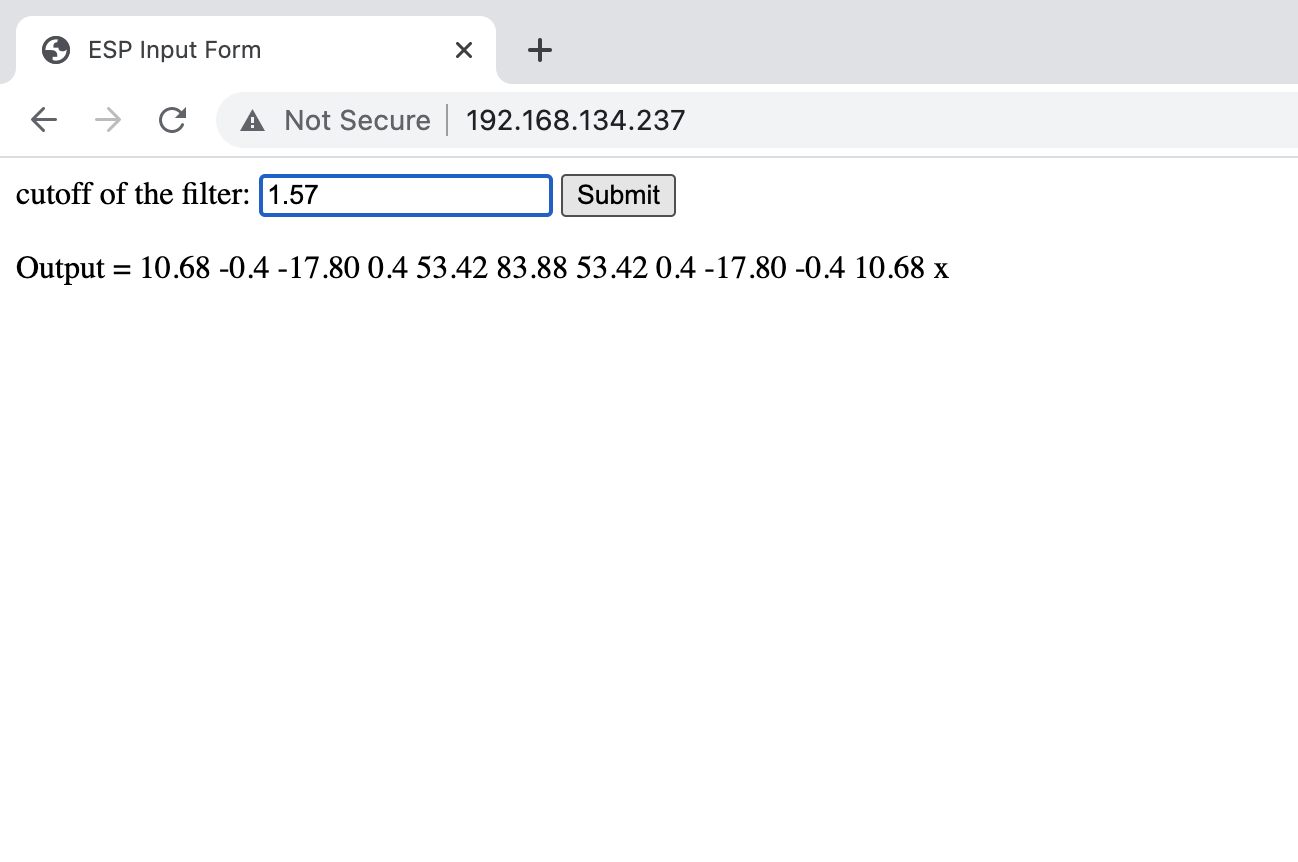
\includegraphics[width=\columnwidth]{interface.png}
\end{figure}
\item Plotting the magnitude response, phase response and impulse response of the filter coefficients. The responses are shown below.
\item The magnitude and phase response show the design filter is a Low pass filter. 
\begin{figure}[H]
	\centering
    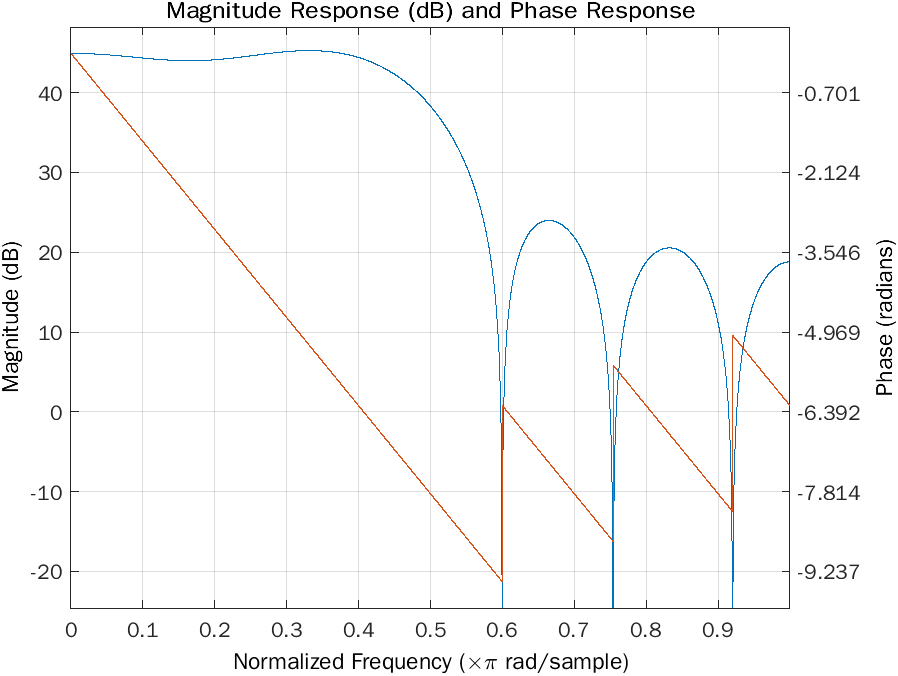
\includegraphics[width=\columnwidth]{mp.png}
\end{figure}
\item Blue gives magnitude response and red gives phase response.
\begin{figure}[H]
	\centering
    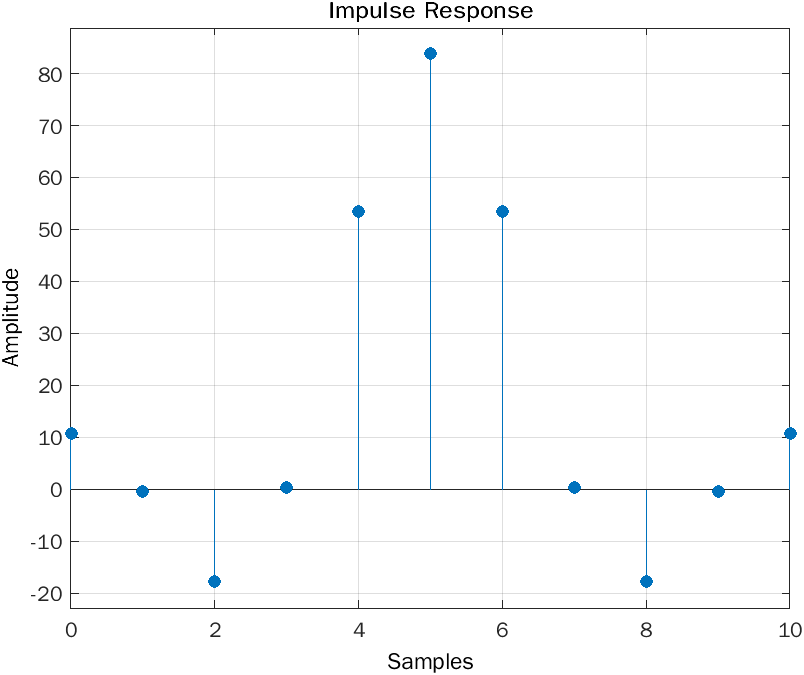
\includegraphics[width=\columnwidth]{i.png}
\end{figure}
\end{itemize}
\begin{thebibliography}{00}
\bibitem{b1} John G. Proakis and Dimitris G. Manolakis, "Digital Signal Processing, Principles, Algorithms and Applications", $3^{rd}$ edition.
\end{thebibliography}
\end{document}